% https://www.overleaf.com/read/jydxqkkkskzp
% https://github.com/MCG-NKU/NSFC-LaTex
% by Ming-Ming Cheng https://mmcheng.net

\documentclass[12pt]{article}
\usepackage[UTF8]{ctex}
\usepackage{nsfc}

\newcommand{\note}[1]{\textcolor[rgb]{0.6,0,0}{note: #1}}
\newcommand{\todo}[1]{{\textcolor{red}{\bf [#1]}}}
\newcommand{\myPara}[1]{\paragraph{#1:}}

\graphicspath{{figures/}}


\begin{document}



%%%%%%%%% TITLE

\title{报告正文:危化品智能装配中的高精度6D姿态估计方法研究}

\maketitle

\ContentDes{(一)立项依据与研究内容(建议8000字以下):}


\NsfcSection{1}{项目的立项依据}{
(研究意义、国内外研究现状及发展动态分析,需结合科学研究发展趋势来论述科学意义;或结合国民经济和社会发展中迫切需要解决的关键科技问题来论述其应用前景。
附主要参考文献目录);}

\subsection{研究意义}

爆炸品、有毒化工、放射性物质、生物化学制剂等危化品的装配工艺,对于制备环境要求很苛刻。工厂装配过程中,为了确保装配安全性,对产线工人的年龄、工作时间和操作流程等都有严格的要求。以工程炸药制备公司为例,为了保障安全生产,工人正常上工前需培训6个月,每天工作时间不能超过6小时,每项工艺流程需双人确认。这些安全措施极大限制了工厂的产能,亟需通过智能制造技术替代人工,提升产能。

% 此处表述6D姿态估计是智能装配中的关键技术,为了提升精度,需要用多传感器融合
待装配物件的六自由度(6D)姿态估计是智能装配的关键技术,其核心问题是高精度的姿态估计。与普通的工业自动化设备不同,危化品的装配操作流程裕度很小,无法通过降低机械操控设备的控制精度和重访精度实现无人操作。智能装配工艺通过装置在产线上的传感器,估计炸药、放射性元素、腐蚀性药品等空腔的姿态,在操控链路形成负反馈,精准完成原料装填和定位螺丝的紧固。

% 传统的6D姿态估计采用RGB或RGBD的方式计算姿态,准确度以目标物体点云的10%作为度量,无法满足精准装配的需要,亟需改进;当前的学术研究中,6D姿态估计算法估计的准确度以目标物体点云尺度的10\%作为度量,其精度只适用于普通物件如快递包裹、日常物品等的粗抓取,无法满足危化品装配的精细操控要求。
面向危化品智能装配的6D姿态估计需要解决三个核心问题,其一为弱纹理表面的算法适应性问题,其二为有遮挡情况下的鲁棒估计问题,其三为姿态估计的高精度修正问题。本项目融合双目相机和光谱相机的影像特征,通过分析多模态传感器数据的特征表达,提取和对齐不同模态的特征,并通过交叉验证抑制单一模态中的噪声,融合有效的互补信息,提升6D姿态估计的适应性、鲁棒性和精度,解决危化品智能装配中的高精度姿态估计难题。

\subsection{国内外相关工作}

大多数姿态估计方法遵循两阶段的范式,首先检测图像中的目标物体,之后在缩放后的目标物体区域上进行姿态估计。尽管现有方法在大多数简单的场景下表现良好,但由于所使用的检测器对弱纹理或被遮挡工件的检测效果并不理想,算法在智能装配应用中的性能急剧下降。

对于第一阶段的目标检测任务,常用的检测方法有两段式和单段式两类\cite{ATSS, fcosv1, fcosv2, PAA, faster-rcnn, maskrcnn}。两段式检测方法首先采用区域建议网络~\cite{faster-rcnn, maskrcnn}生成边界框候选体,然后由分类和细化网络处理,去除假阳性,并调整边界框的位置和大小。这种策略准确度较高,但成本高,效率低。单段式检测器通过在编码器的最终特征图中的每个空间位置用一组预定义的锚框代替区域建议网络来解决这个问题~\cite{retinanet,fcosv1,yolov1}。这种方法会导致锚点中存在大量负样本,虽然这一问题可以通过focal loss~\cite{retinanet,fpn}在一定程度上解决,但程度有限,早期的单段式检测器并没有达到两段式检测器的精度。Zhang~\cite{ATSS}通过一个简单而有效的正样本策略解决了这一问题。最近的大多数检测方法都遵循类似的策略~\cite{fcosv2, PAA, autoassign, OTA, TTF, yolov3},相关改进算法的准确性比两段式方法更好,同时效率更高。但即便如此,这些方法都假设场景中物体的纹理相对丰富,且具有较少的遮挡,与智能装配的6D物体姿态估计场景中的特性仍有较大差异。

% 弱纹理物体位姿估计解决方案:在数据输入源头上解决,即增加depth图像和高光谱图像,实现多源融合。
危化品工件的表面大多没有纹理,这种工况下的目标检测是姿态估计中的一个难点。仅通过RGB图像估计的位姿精度不高,鲁棒性较差。一方面,深度学习网络很难从单幅RGB图像中提取有效的颜色和几何特征,另一方面,三维物体到二维像平面的投影过程丢失了三维结构的几何约束,单幅图像无法逆推结构信息。
基于RGB-D的6D位姿估计方法可以利用点云的三维几何特征来预测目标姿态,其估计精度比单幅RGB图像更高。这类算法的难点在于RGB图和深度图两种异构数据的融和。目前解决的思路有三类。
第一类为像素级融合方法,先利用2D检测或分割网络提取RGB图像特征,将图像特征传递给深度图生成的点云,然后将增强后的点云反馈给点云3D目标检测器。2D检测的结果可辅助三维点云形成3D视锥\cite{Qi2018},减小候选区域的范围。所形成的的视锥也可以进一步划分为网格单元\cite{Wang2019}进行3D检测。或者2D分割的结果也可用于增强3D点云\cite{Vora2020},将增强后的点云输入3D目标检测器提升检测效果。这类方法以顺序的方式进行融合,效率相对较低。
第二类为特征级融合方法,在基于点云的3D目标检测器的中间阶段融合图像和点云特征。例如,在基于网格的检测网络骨干的中间层中使用连续卷积\cite{Liang2018, Liang2019}、混合体素特征编码\cite{Sindagi2019}或Transformer\cite{Zhang2022}网络等融合算子进行多模态融合。
第三类为决策级融合,将RGB图像和Depth图像生成的点云数据通过两个独立网络分别生成2D和3D检测框\cite{Asvadi2018}并融合输出。这种方法可以更好地借鉴每个独立任务的SOTA算法,避免中间特征层上的信息交互,执行效率高,但无法利用不同模式的互补语义信息\cite{Pang2020}提升检测精度。

%本项目在特征级融合的基础上,引入UV数据保持深度图点特征三维空间位置的一致性,从而在异构输入源之间解决视角对齐的问题。
与普通工业零件不同,危化品工件中通常有危险度较高的化学部件,如易爆、有毒或有辐射的填充物。对于这类区域的精细检测和分割,一方面可以避免误操作减少事故,另一方面可为检测网络提供更精准的边界区域特征。不同的化学元素在特定的光谱谱段有脉冲响应特性,可通过光谱相机清晰地定位物质边界,能显著提升姿态估计第一阶段的检测和分割精度。光谱图像的检测和分割算法思路与可见光图像相似,最主要的问题在于样本数据较少,且分布不均匀,业界没有大规模数据集可用于网络训练。目前解决这一问题的主要方法是小样本学习\cite{lys2022targetDetection, shi2020HyperspectralTargetDetection}或加强注意力机制\cite{shi2020hyperspectralROI}。

% 此处描述 RGB, Depth, 和光谱数据融合的国内外现状
对于同一场景下的可见光、深度图和光谱图像的融合处理,目前没有可直接借鉴的方法,但多传感器融合的方法在遥感影像处理和自动驾驶领域中都有相关研究。一种朴素的融合方法是决策级融合,对不同的输入数据分别提取特征图\cite{pang2020clocs},构建基于统计的特征加权组合模块,对不同输入分支提取的特征赋予不同的权重,在输出层进行决策级融合\cite{li2022sal}。这种方法既可以区分不同输入源特征在分类器中的重要性,又可以避免特征提取网络学习本身对分类结果的干扰。但它没有考虑多源数据特征间的差异性与互补性。另一种思路是特征级融合,先前的研究有两种模式,其中一种模式以Xie等人提出的Pi-rcnn\cite{xie2020pircnn}和Vora等人提出的Pointpainting\cite{vora2020pointpainting}为代表,将三维点云中的每一个点投影到二维像平面,然后通过双线性插值获得对应二维图像特征。这种方式虽然在像素级进行了细粒度的特征聚合,但是该操作过程由于融合点的稀疏性而失去二维图像密集特征的优势,即破坏了二维图像特征的语义一致性。另一种方式以Chen等人提出的MV3D\cite{chen2017multi}为代表,利用3D目标检测器分别获取点云数据和二维RGB图像中初始建议框,然后融合两种模态感兴趣区域特征。这种方式通过实例级融合保持了语义的一致性,但是利用3D目标检测器获取初始建议框的阶段所提取的特征相对粗糙,且缺失二维图像中的稠密信息表征。

% 在对不同输入源的数据进行特征抽取时,增加三维交叉注意力模块\cite{li2022triplet}增强多源数据的互补空间特征,并进行逐层特征融合。这种方法在自动驾驶领域\cite{huang2020epnet}取得了不错的结果。\note{补充特征级融合的问题}先前的研究有两种模式:一是将三维点云中的每一个点投影到二维的像平面,然后通过双线性插值获得对应的二维图像特征。这种方式虽然在像素级进行了细粒度的特征聚合,但是该操作过程由于融合点的稀疏性而失去光谱图像密集特征的优势,即破坏了二维光谱图像特征的语义一致性。另一种方式是利用3D目标检测器分别获取点云数据和光谱图像中初始建议框,然后融合两种模态感兴趣区域特征。这种方式通过实例级融合保持了语义的一致性,但是利用3D目标检测器获取初始建议框的阶段提取的特征相对粗糙且缺失光谱图像中的稠密信息表征。


% 有遮挡情况下的鲁棒估计现状
遮挡是6D姿态估计中的另一个难点问题,通用的目标检测方法假设物体之间遮挡较少,标准真值包围框中心的区域周围为目标物体,因此在网络学习中专注于仅从这些区域提取的样本预测边界框参数。然而,在有遮挡的情况下,真值包围框的中心通常被其他物体或者场景元素遮蔽,导致检测框出现较大偏差。为了提升姿态估计的性能,大多数方法需要依赖额外的姿态修正组件。这些组件首先根据初始姿态以及物体的CAD模型渲染合成图像,然后基于光流网络估计渲染图像和输入目标图像之间的密集2D-to-2D对应关系。在利用目标的3D形状信息将2D对应关系提升到3D-to-2D对应关系之后,基于PnP算法迭代计算更精细的姿态参数。

这种算法框架在大多数通用场景下表现良好,但它有几个缺点。
首先,所使用的光流网络建立在两个假设之上,即两个潜在匹配之间的亮度一致性和本地邻居内匹配的平滑度。这一假设在通用场景下是成立的,但在智能装配的6D物体姿态估计场景下,我们没有关于目标形状的线索,缺少形状约束,从而导致目标图像中每个像素的潜在匹配空间盲目扩大。
其次,匹配过程中物体形状信息的缺失会导致匹配结果出现明显偏差,在PnP姿态求解过程中引入显著噪声。
另外,在这种两阶段的框架中,第一阶段的训练依赖于匹配网络的损失函数,该匹配损失不能直接反映最终的6D姿态估计损失,且不是端到端可训练的。

近几年的位姿估计方法,通过使网络预测一些预定义的3D关键点~\cite{rad2017bb8, hu2019segDriven, peng2019pvnet, Hu2021},或对每个2D像素预测稠密的对应3D点~\cite{zakharov2019dpod, Su2022, li2019cdpn, wang2021gdrnet, Di2021}来创建对应关系。之后通过数值PnP求解器~\cite{lepetit2009epnp}或直接从中间对应关系的表达来学习姿态~\cite{hu2020singleStage, EroPnP,wang2021gdrnet, Di2021}。通过精心设计卷积神经网络结构改进的算法~\cite{he2016resnet, resnext_2017_cvpr}在鲁棒性和准确性方面都有显著提升~\cite{Xiang2018, peng2019pvnet, wang2019densefusion60},但复杂的杂乱场景下,姿态估计的准确性依然不高。

对于6D姿态的修正,以往的方法主要依赖于已配准的深度图~\cite{Xiang2018, li2019cdpn, wang2019densefusion60},但在许多真实场景~\cite{Hu2021}中深度图难以直接获取。
近几年的姿态修正方法使用无需深度数据的“渲染-比较”策略,可以获得性能相当或更好的结果~\cite{li2018deepim, zakharov2019dpod, cosypose, rad2017bb8, Hu2022, Lipson2022, RNNPose_2022_cvpr,Repose_2021_iccv}。Hu等~\cite{Hu2022}近期提出的6D姿态修正方法与这一策略有所不同,他将6D姿态修正问题建模为渲染图像到目标图像之间的2D匹配关系问题,通过数值求解获得修正之后的姿态。算法精度比“渲染-比较”的策略更高,但由于该方法将6D姿态修正建模为无约束的纯2D到2D匹配问题,脱离了6D物体姿态的物理意义,因此理论上讲估计结果是次优的。为了提升性能,申请人团队提出了一个由目标的3D形状引导的形状约束递归匹配框架,在精度和效率方面都有了大幅提升\cite{?}。

% 为了解决当前检测器在遮挡环境下的退化问题,我们提出了一种检测方法,该方法利用了6D姿态估计中目标对象是刚性的这一特性。
% 对于此类对象,任何可见部分都可以提供完整边界框的可靠估计。因此,我们认为,与标准物体检测器使用的基于中心的采样相比,任何从可见部分提取的特征都应该是训练期间正样本的潜在候选。
对于危化品智能装配中的三个核心问题,每个细分学术领域的学者及申请人团队都有相关的基础研究。在多模融合解决弱纹理物体的检测方面,可见光和深度图像融合估计已有可借鉴的算法框架,但如何有效融合光谱数据仍需探索。有遮挡下的鲁棒估计是目前6D姿态估计中的一个公认难题,通过改进网络结构和融合策略提升鲁棒性目前算法改进的主要思路。而对于高精度姿态修正问题,基于几何引导的约束框架是目前探索的行之有效的解决方案,但仍有很大的改进空间。

{
\bibliographystyle{IEEEtran}
\bibliography{nsfc_sr}
}


%%%%%%%%%%%%%%%%%%%%%%%%%%%%%%%%%%%%%%%%%%%%%%%%%
\NsfcSection{2}{项目的研究内容、研究目标,以及拟解决的关键科学问题}{
(此部分为重点阐述内容);}

\subsection{研究目标}

针对危化品智能装配中6D位姿估计中的工件表面弱纹理、工件叠放有遮挡和位姿估计精度不满足自动化操控需求这三个核心问题,研究融合可见光、深度图和光谱图的检测和姿态估计深度学习网络,分析智能装配场景下影响目标检测准确度和姿态估计精度的因素,从网络结构、损失函数和融合策略等方面改进算法,提升工件姿态估计的精度,满足危化品智能装配对工件姿态估计精度的要求。预期发表学术研究论文15篇,其中顶会或顶刊论文10篇,申请专利和软件著作权10件。

\subsection{研究内容}

% 0. 总述
分析双目可见光和光谱相机数据的匹配关系,研究互补融合表征的方法,解决工件表面弱纹理情况下的目标检测问题;研究刚性物体的感知检测网络结构,提升有遮挡情况下的目标检测精度;改进基于CAD模型几何特征引导的姿态修正模块,提升姿态修正的准确度。对三个分支的改进策略在不同网络层级进行融合,研究高效复合的深度学习网络,提升工件6D姿态估计的精度。主要研究内容包括以下三部分:
% --- 参考
% 为了解决同类研究在真实复杂环境下暴露的不足,本课题组研究涉及危险设备智能装配环境下基于几何特征引导的目标六自由度姿态估计问题,并融入多源融合表征以及多模态3D目标检测框架。研究内容可提炼为三个方面,它们互相联系构成完整的面向危险设备智能装配零部件的六自由度姿态估计系统。

% 1. 可见光、深度图和光谱图的特征融合方法
1. 面向弱纹理工件的目标检测任务,研究多模态影像数据的融合表征方法。研究不同模态数据特征的提取和对齐方法,分析在不同空间尺度和特征层深度进行信息交叉对弱纹理工件检测结果的影响,以及对等网络结构和主从式融合网络结构对位姿估计结果的影响,通过原理分析和实验验证探索危化品装配中对弱纹理工件检测任务的最佳多模融合方法。

% --- 参考
%\textbf{A、面向危险设备智能装配零部件的多源融合表征}
%针对危险设备智能装配零部件的多源融合表征多模态对齐融合的问题和挑战,以融合方案对位姿估计优化后的精度为评价依据,研究多模态信息的表达和特征提取。研究该过程包含两个细节问题:(1)针对目标数据的差异性以及不同模态数据对于姿态估计任务的重要性,解决姿态估计问题中多种信息表达的关键问题,制定高效针对性的目标特征提取策略;(2)研究神经网络下多模态特征的信息对齐和融合问题,提出可行的多模态信息融合方式。


% 2. 有遮挡情况下的目标检测精度
2. 有遮挡情况下的刚性工件目标检测精度提升方法。研究如何利用目标边界框中的所有3D空间信息指导生成可见性掩膜,避免场景元素遮挡下掩膜不可用的问题。研究如何使用可见性掩膜指导网络训练时对候选目标的抽样,使网络参数训练过程仅由可见部分监督,避免遮挡部分的干扰。分析通道融合策略,通过融合多个可靠局部区域的预测结果,提升工件整体检测的准确度。

% --- 参考
%\textbf{B、针对危险设备智能装配零部件复杂环境下的3D目标检测}
%主流的目标检测算法在通用数据集上可以实现高精度、高实时性的目标检测。这类方法通常使用特征金字塔网络(FPN)来输出比例丰富的特征图,然后将每个特征向量作为训练样本,由分类分支和回归分支进行进一步处理。这类框架成功的关键在于训练期间选择正样本并且假定真实边界框中心的区域能够提供目标信息,即不被其它物体遮挡。然而在工业零的部件所处的复杂环境中,目标经常受到严重遮挡,无法满足中心假设。另外,常规的目标检测算法没有考虑使用刚性目标的可见部分为边界框的预测提供信息。针对以上问题和挑战,本课题将研究一种刚性感知检测方法来提高目标检测精度。具体包含三个以下问题:第一,如何利用目标边界框中的所有像素信息来指导生成可见性掩膜,避免场景元素遮挡下的掩膜不可用的问题;第二,如何使用可见性掩膜指导训练期间对候选目标的抽样,使得网络由所有可见部分监督并且丢弃遮挡部分;第三,如何融合所有高可靠性候选局部预测,以产生更加鲁棒的检测结果。0



% 3. 基于几何引导的姿态修正
3. 基于工件几何特征引导的位姿修正方法。基于CAD模型将工件的几何特征在每一次迭代的位姿下进行投影,分析和设计有效的网络结构和注意力机制,将几何信息引入目标图像与渲染图像的特征匹配过程,对6D姿态误差损失函数进行精细化设计,提升每次迭代的度量精度。


% --- 参考
%\textbf{C、面向工业机械臂抓取基于零部件CAD模型几何特征引导的目标六自由度姿态估计网络设计}
%基于检测-估计-修正的6D姿态估计框架显示出了优良的性能,被近期提出的大多数方法所采用。采用一个单独的6D姿态修正网络可以放松对前一级估计网络的要求。同时基于CNN的6D姿态修正网络的输入为目标图像与在前一级估计网络得到的粗糙姿态下的渲染图像,这样的输入可以减轻姿态修正网络对数据的需求。目前大多数方法通过估计目标图像与渲染图像之间的对应关系来求解目标图像中物体的6D姿态。然而这种方法很强地依赖于物体的纹理特征,而对于工业零部件,大部分物体呈现出弱纹理或者弱纹理的特征,因此这种方法应用于工业零部件上会有很强的局限性。因此对于弱纹理或者弱纹理的工业零部件,物体的几何特征需要被有效地利用,然而现有的姿态修正方法很少探索物体的几何特征。
%本课题拟提出一个基于物体几何特征的6D姿态修正方法。在现有的基于纹理特征的对应关系估计网络中,如RAFT,本文通过利用点云特征提取网络,显式地将物体的几何特征进行编码,作为对应关系估计网络的参考信息。在迭代优化过程中,对应关系估计网络全局地通过可微姿态求解层来修正在上一步迭代过程中求解得到的姿态。具体来说,将物体的几何特征在上一步估计得到的姿态下进行投影,同时将物体的几何信息引入目标图像与渲染图像的特征匹配过程中,结合特征匹配结果与投影得到的几何特征来全局地求解更新之后的目标物体的6D姿态。



\subsection{拟解决的关键科学问题}

1. 弱纹理工件的可见光、深度图和光谱图的有效融合表征问题。在弱纹理条件下,光谱数据可捕获准确的材质信息,为基于可见光图像和深度图的区域分割提供稀疏但可靠的先验,但如何充分挖掘深度图和光谱数据对可见光图像特征提取的引导和补偿,实现多模态数据在姿态估计任务中的协同表达是本课题需要解决的关键科学问题。

2. 有遮挡情况下的工件3D目标检测鲁棒性问题。智能装配场景中工件存在相互遮挡的情况,基于目标中心区域抽样进行估计的方法不再适用。尽管理论上可以将该问题拆分建模为目标分割任务,通过标注以及目标物体掩膜估计来区分目标前景以及背景,但像素级的掩膜标记成本过高。与常规目标检测任务不同,装配流程中的危化品通常为刚体,如何利用这一特性降低掩膜标注的要求,提高检测鲁棒性,是3D目标检测中的关键问题。

3. 位姿修正中的工件CAD模型几何特征引导问题。当前算法中6D姿态修正都依赖物体表面的纹理,对于弱纹理工件,这一方法不再适用。现有的姿态修正方法已将3D问题通过渲染技术转换成无约束的2D匹配问题,搜索空间巨大,严重制约匹配的精度和效率。如何在位姿修正的2D匹配中引入3D几何约束,提高姿态修正精度,是本课题要解决的关键问题之一。

% --- --- --- --- --- --- --- --- --- --- --- --- --- --- --- --- 
% 以上内容,2023-2-27 17:14:04 SR已修改

\NsfcSection{3}{拟采取的研究方案及可行性分析}{
(包括研究方法、技术路线、实验手段、关键技术等说明);}

\subsection{拟采取的技术路线}
本课题研究的面向危险设备智能装配零部件六自由度姿态估计的总体方案示于图\ref{fig:sys_arch}。其中涉及的三个关键问题的详细方案和可行性分析分别阐述如下:

\begin{figure}[h]
	\centering
    \begin{overpic}[width=0.8\columnwidth]{sys_arch.png}
    \end{overpic}
    \caption{本课题研究方案的总体框架
    }\label{fig:sys_arch}
\end{figure}


\textbf{A.空间-语义联合一致性的多源融合表征设计方案}

\begin{figure}[h]
	\centering
    \begin{overpic}[width=0.8\columnwidth]{feature_biflow_fusion.png}
    \end{overpic}
    \caption{特征级双向全流多源融合
    }\label{fig:feature_biflow_fusion}
\end{figure}

% 融合方案的整体描述
本项目针对危化品智能装配环境提供的真实数据集,以双目相机为主传感器,光谱相机为辅助传感器,构建主从式融合网络架构,设计异构数据间的特征提取与共享机制,从而实现多源数据的空间对齐和语义聚合,为后续的3D目标检测和6D位姿估计等下游任务提供多源融合特征。

%首先,在真实危化品装配环境下,通过双目相机和光谱相机采集真实场景下的RGB图像、Depth图像和光谱图像,研究各模态数据的差异性以及各模态数据的合理表达。RGB图像做空间变换时,由空间三维坐标和相机相平面坐标构建的投影方程将不再成立。为了保持空间位置信息的一致性,本项目拟在RGB图像通道维融合像平面UV坐标数据作为编码器的输入。另外,Depth图本身表示的是物体上的点到相机的距离,这种距离在三维空间的表达就是物体姿态的一种体现。早期的一些方法将Depth图像当作二维信息处理,作为类似灰度图的单通道图像提取特征,或者直接融合到RGB图像中,将3通道的RGB图像转换为4通道的RGB-D图像。虽然这种操作在一定程度上较优于仅使用RGB的方式,但是该操作忽略了Depth图像中的三维结构信息。所以本项目拟将Depth图像的深度信息通过相机内参转换为三维点云信息,使用点云网络提取目标的姿态和距离特征。

% 然后,利用CNN或Transformer分别提取融合UV的RGB图像和光谱图像数据的语义特征和光谱特征,利用点云网络(Point Cloud Network,PCN)提取点云特征。当语义特征、点云特征和光谱特征信息在三个网络分支上流通时,研究语义特征和点云特征,点云特征和光谱特征两两之间的对齐融合机制。

% 针对语义特征和点云特征信息流的对齐融合过程,本项目拟以由Depth图像转换的三维点云形成的XYZ图为桥梁,设计一种查询算法,例如最近邻算法或其变种算法,对Depth图像中每一个特征点在XYZ图中找到最近的三维特征点,然后通过最大池化或多层感知机等模块聚合对应位置的RGB图像的语义特征。该过程中有一个值得注意的问题是,在RGB图像分支语义特征编码阶段,随着网络深度的加深,语义特征图的高度和宽度就越小。为了RGB图或Depth图各特征点以XYZ图为桥梁的映射过程中依然能够找到对应的三维特征点,本项目拟设计一种动态缩放机制,例如最近邻插值算法或其变种算法等,使得语义特征与点云特征在编码阶段映射到XYZ图中始终能维持空间维度对齐。

% 针对点云特征和光谱特征信息流的对齐融合过程,本项目拟在先前研究的基础上,通过一个可学习的对齐特征图为桥梁,以数据驱动的方式建模光谱图像与3D点云不同模态间的对齐匹配关系。为了保留光谱图像数据中目标的具体细节特征,本项目拟设计一个交叉注意力特征对齐模块,对点云编码后的点云特征点查询稀疏编码后的光谱向量,得到逐像素的语义对齐图,然后将语义对齐图聚合到点云特征信息流中。为了便于更好的学习点云与光谱图像的语义一致性,本项目拟提出一种自监督交叉模态损失函数。首先使用配对的二维和三维建议框提取光谱图像和点云的原始特征,然后在二维和三维空间中对建议区域进行相似性损失监督,增强交叉注意力特征对齐模块的语义感知能力。

% % 重点1:与之前方法不一样的地方在于,不是通过确定的相机内参匹配2D图像和3D点云,而是通过一个可学习的对齐特征图为桥梁,以数据驱动的方式建模2D图像与3D点云不同模态间的对齐匹配关系。

% 最后,通过RGB图像,Depth图像和光谱图像三模态三条支路融合提取的语义特征,点云特征和光谱特征级联在一起得到最后的融合特征用于下游任务,例如3D目标检测和6D姿态估计。


\textbf{B. 针对危险设备智能装配零部件复杂环境下的3D目标检测网络设计方案及可行性分析}(王庆元)
\begin{figure}[h]
	\centering
    \begin{overpic}[width=0.8\columnwidth]{visable_guided_3d_detection.png}
    \end{overpic}
    \caption{可见性引导的3D目标检测流程图
    }\label{fig:visable_guided_3d_detection}
\end{figure}

该关键问题的研究重点着眼于危化品智能装配环境下目标刚体存在的严重遮挡问题,设计了一种基于刚体感知的2D和3D目标检测器,并将2D检测结果用于指导3D目标检测器以获得更准确的3D检测结果,如图~\ref{fig:visable_guided_3d_detection}所示。

现有的单阶段2D目标检测方法专注于学习仅从真实边界框中心区域抽取的样本来预测边界框参数,当目标中心被其他对象或场景元素遮挡时将无法提供精确的检测结果,对于复杂场景下工业零部件的目标检测并不适用。由于6D姿态估计中的目标对象通常是刚性的,这类目标的所有可见部分都可以为边界框的预测提供可靠的估计,因此本方案提出了一种刚性感知检测方法,具体包含以下三步:第一步,获取真实对象的掩膜。通常这种掩膜在目标受到场景元素遮挡的情况下是不可用的且价格昂贵。为了避免使用这样的掩膜,提出了一种距离变换图来获取可见部分的掩膜。该方法先对真实刚性目标2D边界框进行裁剪来得到图像块,依据刚性目标的可见部分与边界部分像素值之间的显著差异性,设计了一种可见性距离函数用于计算图像块内所有像素与边界之间的距离,以此构建目标的可见掩膜;第二步,获取候选正单元。首先使用主干网络对融合特征进行特征提取来生成特征图。依据每个特征单元对应所有像素的可见性距离来计算特征单元的可见性分数,设置可见性分数阈值对所有的特征单元进行筛选采样以获得候选正单元。然而,使用全部的大于阈值的正单元将导致训练过程被较大的目标所支配。为了避免这种情况,我们根据阈值为每个目标对象实例随机选择一定数目的正单元,对于少于该数目前景单元的实例进行多次随机采样。最后,丢弃未被选为正样本的单元以避免其向网络提供潜在不一致的监督信号;第三步,融合候选预测。通常在推理过程中每个对象实例通常会收到多个框预测,现有方法使用非最大抑制来选择局部区域内有最大置信度的候选框。然而,这种方法依赖于靠近边框中心的小区域来提供高精度预测。本方案通过将邻域中的所有候选框组合在一起,来获得更准确的结果。为此,我们让特征单元预测一个额外的置信值,表示预测框的精确度。然后,我们对具有相同局部最大值的不同局部预测进行聚类,并将它们分配给相同的对象实例。最后,通过一个简单的加权和来组合同一群集中的所有候选局部预测,并基于预测的置信值进行加权以获得更加鲁棒和精确的检测结果。

对于3D目标检测,本方案设计了一种类似于2D刚体感知检测的方法对目标进行3D框的回归和分类。该方法同样可以分为三步:第一步,获取点云数据的逐点分割掩膜。首先将真实的3D边界框依据相机参数投影为相机平面的2D边界框,然后以2D边界框为参考对点云进行裁剪来得到3D点集。考虑到2D边界框附近的点相对于刚性目标表面的点的深度值存在显著差异,本方案设计了一种深度距离函数用于计算3D点集中的每个点与边界上的点之间的深度距离,以此构建一种柔性的分割掩膜;第二步,获取候选正单元。首先对于每个特征单元,计算该单元对应所有点云的深度距离,并以此距离为依据计算特征单元的得分。设置深度距离得分阈值来对所有的特征单元进行筛选以获得候选正单元。然后采用与2D检测类似的方法,为每个目标对象实例随机选择一定数目的候选正单元以避免训练过程被较大的目标所支配。最后,丢弃所有未被选为正样本的特征单元;第三步,基于2D检测引导的3D候选融合。与2D融合候选预测类似,本方案同样为每个3D候选框预测一个额外的置信度。为了提升3D目标检测的精度,本方案在融合最终的3D候选预测之前,依据2D目标检测候选与3D目标检测候选的几何一致性和语义一致性来生成更准确的3D检测结果。对于几何一致性,我们依据相机参数将3D检测候选框投影到图像平面,并计算所有投影框与2D检测候选之间的交并比(IoU)。对于语义一致性,我们只考虑同类别的2D检测候选来引导3D检测候选。然后,以交并比、2D检测置信度、3D检测置信度以及3D边界框与相机之间的归一化距离作为元素构建2D-3D关联张量。对于该张量,我们选择保留与2D检测候选没有交集的3D检测候选,而去除与3D检测没有交集的2D检测候选,因此该张量为稀疏张量。之后,将该稀疏张量输入到一个轻量级的残差网络中,输出所有3D检测候选融合置信度得分。最后,本方案为了避免非最大抑制方法对正确的检测进行抑制,采用与2D检测类似的方法,通过聚类和加权,将邻域中的所有候选框进行融合以提高3D检测的鲁棒性和准确性。


% \begin{figure}[h]
% 	\centering
%     \begin{overpic}[width=0.8\columnwidth]{rigid_detect_analysis.png}
%     \end{overpic}
%     \caption{刚性检测分析
%     }\label{fig:rigid_detect_analysis}
% \end{figure}
% 我们展示了不同抽样策略的检验精度。在典型的一般对象数据集(COCO[29])和典型的6D目标位姿数据集(YCB-V)上的训练期间,不同的局部预测。图中显示了FCOSv2(Center)、ATSS(Center+)的结果,以及利用真实掩膜中的所有候选框(Visible)策略的结果。水平轴表示局部预测到边框中心的归一化距离。


%下面这一段为可行性分析
一阶段目标检测器通常使用特征金字塔(FPN)输出多种比例的特征图,将特征图中的特征向量作为训练样本进行分类和回归处理。在检测训练期间,需要为每个注释的目标实例定义正样本和负样本,并使用正样本回归目标实例的边界框参数。因此这一框架的关键是在训练期间有效的选择正样本。本课题的前期预研中,使用典型的6D目标位姿数据集(YCB-V)将所提出的刚性感知策略与基准策略进行对比。图~\ref{fig:detecting_rigid_objects}显示了两种策略的采样方式及检测结果。图(a)是基准采样策略,该策略选择目标中心周围的正样本(绿色单元),而此处受到了场景元素遮挡。图(b)是我们提出的可见性引导的采样策略,该策略丢弃了遮挡区域,并且使网络由所有可见部分的监督。采样概率由不同深浅的绿色表示。图(c)显示了我们的方法(绿框)相比基准策略~\cite{Zhang2020}(红框)可以产生更准确的检测结果。本课题将把该方法从2D边界框回归拓展到3D目标检测领域。

\begin{figure}[h]
	\centering
    \begin{overpic}[width=0.8\columnwidth]{detecting_rigid_objects.png}
    \end{overpic}
    \caption{杂乱场景中的刚性物体检测
    }\label{fig:detecting_rigid_objects}
\end{figure}


\textbf{C. 面向危险设备智能装配基于零部件CAD模型几何特征引导的目标六自由度姿态估计网络设计方案及可行性分析(海洋)}


\begin{figure}[h]
	\centering
    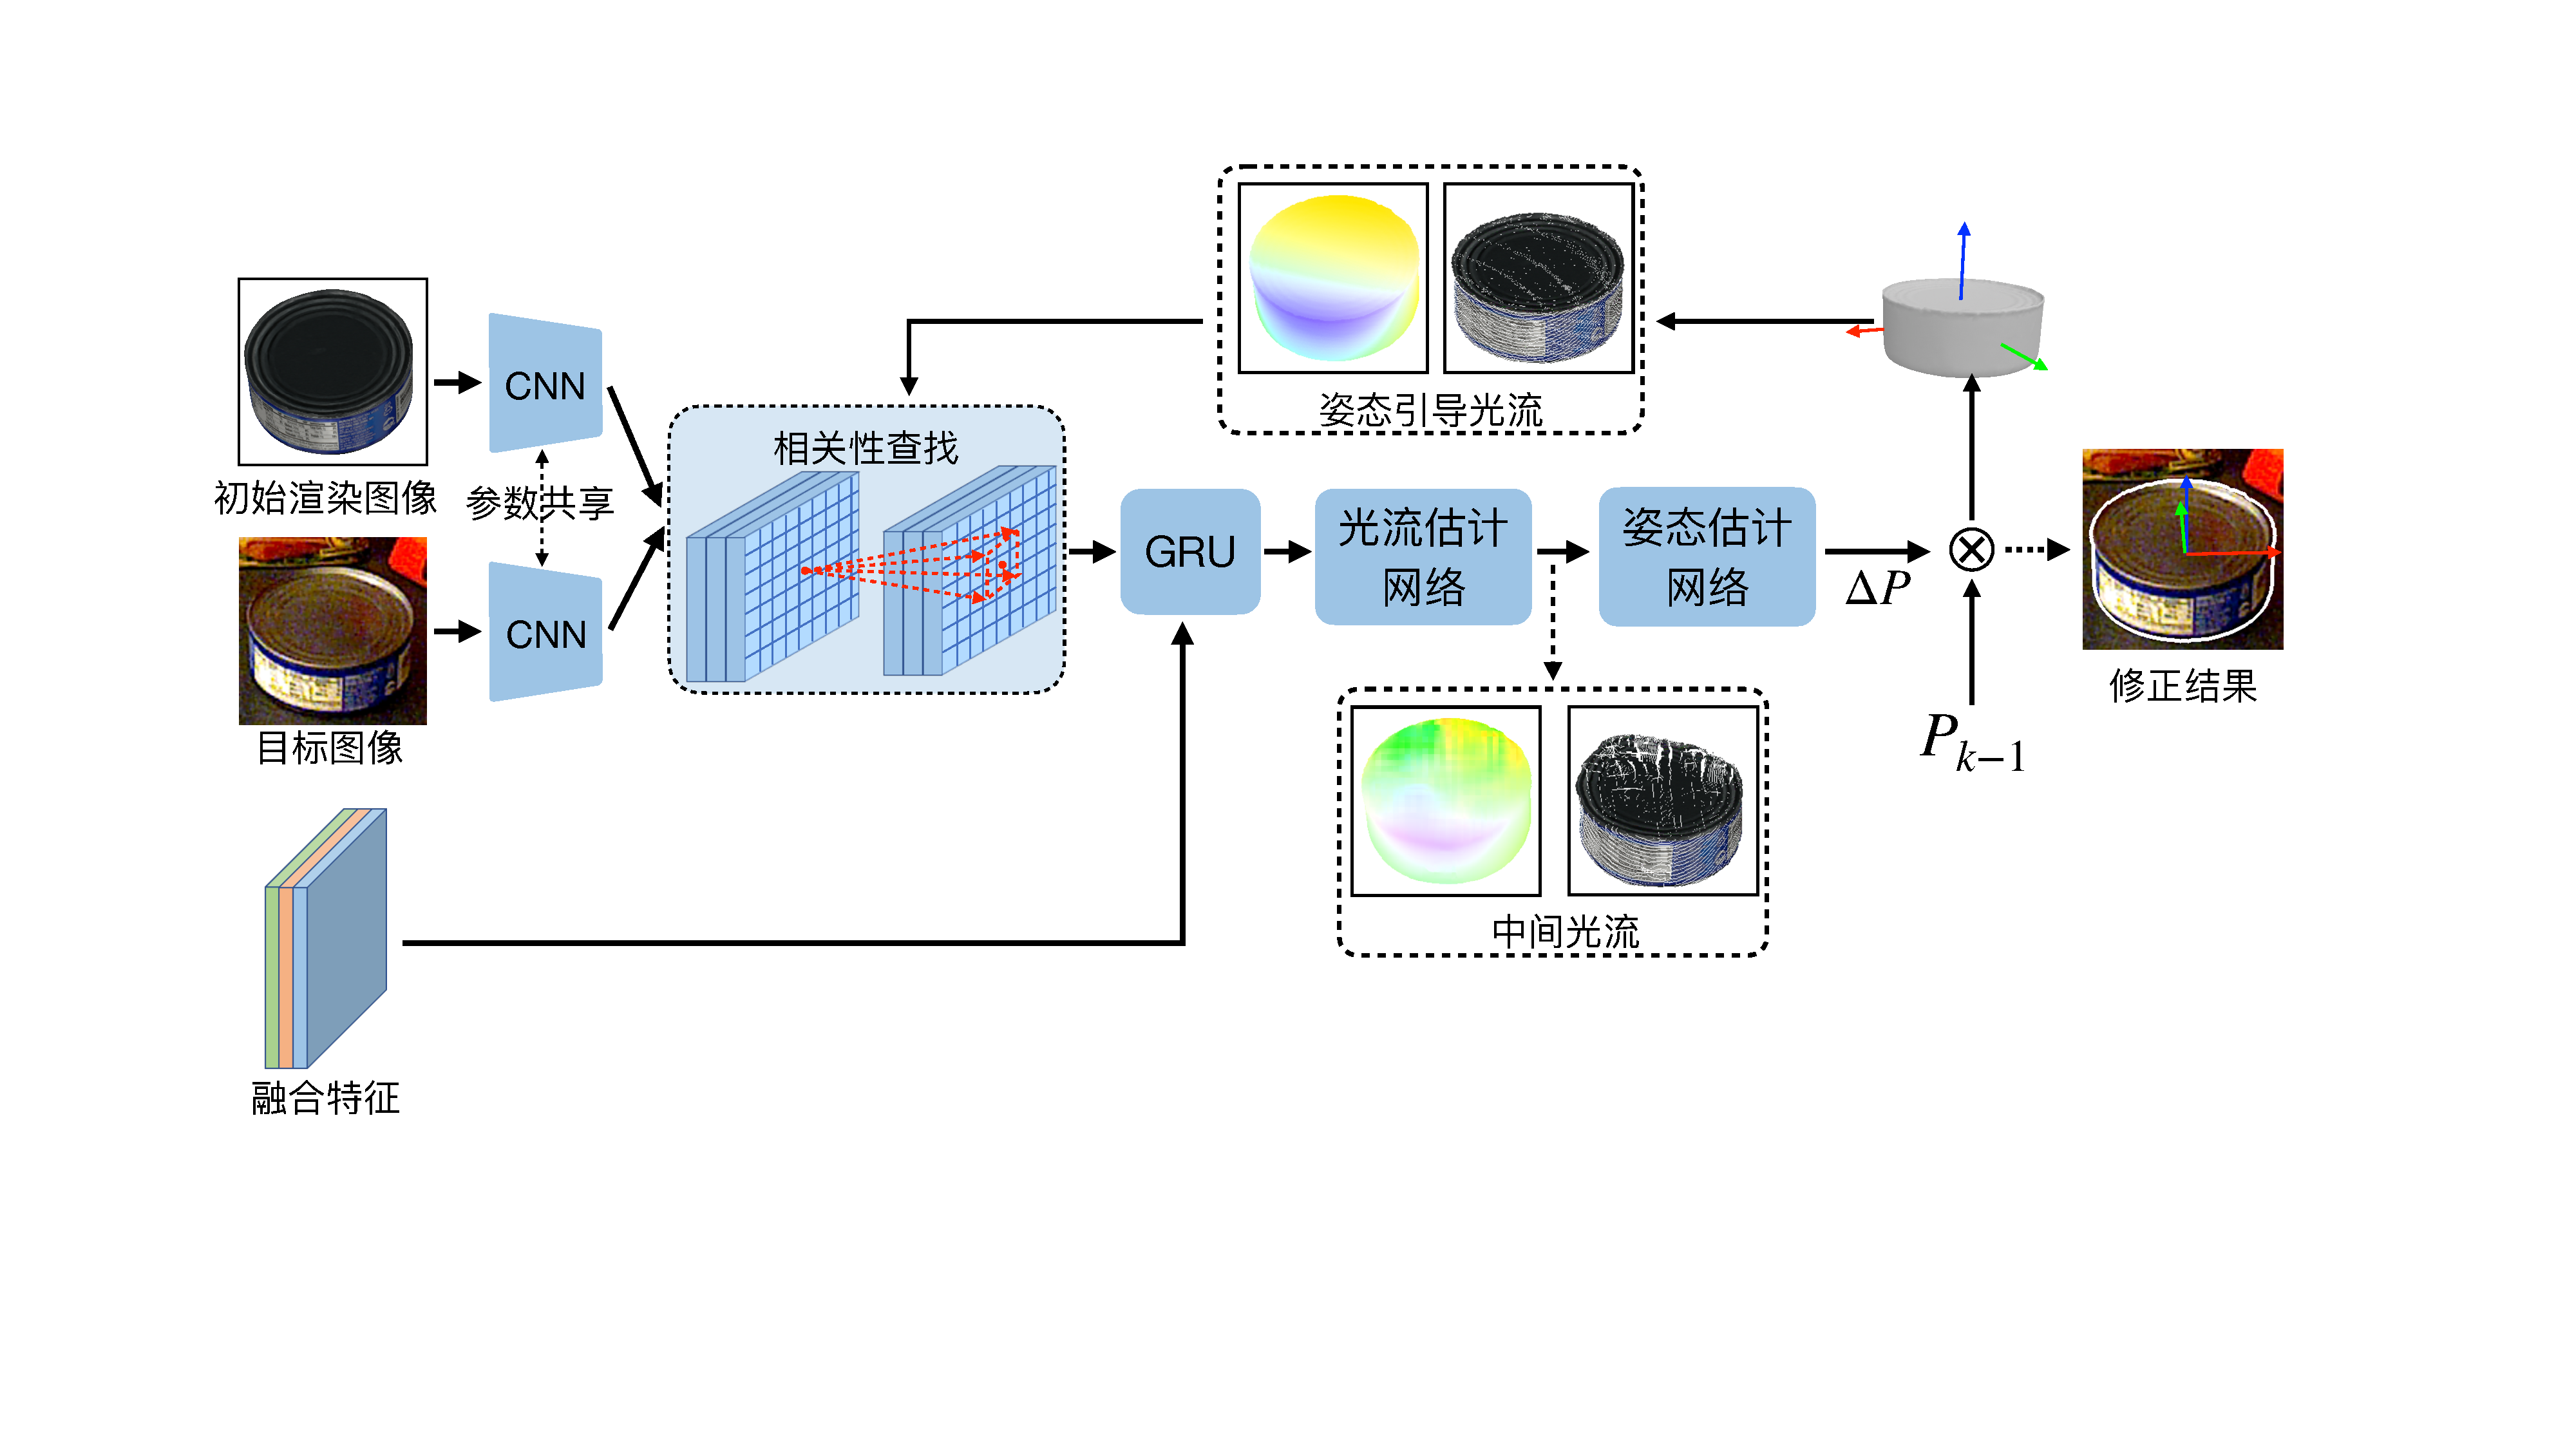
\includegraphics[width=0.9\linewidth]{figures/shape_constraint_flow_arch.pdf}
    \caption{基于几何特征引导的6D姿态修正框架
    }\label{fig:geo_guided_6D_refine}
\end{figure}

本方案的关键问题在于对针对目标物体估计得到的不精确的6D姿态进行修正。目前基于2D匹配的6D姿态估计修正方案主要依赖于物体的纹理特征进行,没有考虑到物体的几何特征,因而不适用于弱纹理的目标。同时,当前方法没有考虑到可以利用物体的3D几何约束来缩小匹配空间。
本方案提出基于几何特征引导的物体6D姿态修正框架,结合多源融合特征,通过物体的3D几何约束,引入物体的几何特征。

如图~\ref{fig:geo_guided_6D_refine}所示,本方案首先利用目前成熟的6D姿态估计网络预测得到一个不精确的6D姿态,然后利用该姿态对目标进行渲染和定位。
之后利用卷积神经网络对目标图像和初始渲染图像分别进行特征提取,并通过两张图像抽取的所有特征向量构造4D相关体。
然后,通过迭代修正6D姿态来逐步提高其精度,其中相关性查找起着核心作用。
相关性查找在4D相关体中在当前估计的2D密集匹配以及其周围邻域中进行索引,进而确定在当前估计的2D密集匹配下的相关性。迭代修正的核心思想即为逐步修正估计的2D密集匹配,使其朝着相关性更高的方向移动。

我们的迭代修正框架建立在GRU上,GRU被证明在序列任务建模中发挥着良好的作用,通过引入门控机制,选择性地保留或者舍弃先前的状态信息。在这里,我们将查找得到的相关性特征与多源融合得到的特征进行拼接,输入GRU中,GRU对其内部的状态信息进行更新。
目前的6D姿态修正方法只利用一个光流估计网络来根据GRU更新后的当前状态信息来估计修正之后的2D密集匹配。然而,如前所述,这一范式只考虑到了物体的纹理特征,不适用于本方案的研究目标。
本方案提出通过使用额外的姿态估计网络,该网络的输入为修正之后的2D密集匹配与GRU的内部状态信息,并通过整合全局的局部对应关系来预测一个反映当前运动信息的相对姿态。
基于此,我们在每次迭代中预测一个相对姿态,通过累加得到最终的修正结果,我们的网络是端到端的,通过基于物体形状的损失函数来直接优化6D姿态,网络可以隐式的感知到物体的3D几何形状。


本方案的核心贡献是通过姿态引导光流来进行相关性查找。如图~\ref{fig:geo_guided_6D_refine}所示,光流估计网络得到的光流无法反映物体的形状,有很严重的畸变。因此我们提出通过能够严格反映物体形状的光流来进行相关性查找,进而在训练过程中,使网络感知到物体的3D几何形状。给定渲染图像的姿态以及当前估计的6D姿态,我们可以通过几何计算得到初始渲染图像中的每个像素在当前估计6D姿态下的对应点,也就是图~\ref{fig:geo_guided_6D_refine}中的姿态引导光流,能够严格反映物体的形状。同时,这种全局感知的方式能够修正一些不可靠的光流估计,进而得到与全局姿态相符合的对应点,进而使得这些像素迅速逃离局部解,缩小匹配时的搜索空间。

\subsection{可行性分析}

\textbf{A.特征级对齐的多源融合表征设计方案的可行性分析}


\NsfcSection{4}{本项目的特色与创新之处;}{}

\textbf{A. 多源融合表征的特色与创新之处}
一方面,通过引入额外的UV数据保持深度图点特征三维空间位置的一致性,由此可通过参数共享的神经网络架构,在RGB和Depth特征提取阶段,通过全流双向融合各自互补特征。另一方面,通过引入光谱图像,针对危险设备智能装配零部件不同地光谱特征响应,可以更准确和鲁棒地提取装配零部件实例级目标特征。

\textbf{B. 3D目标检测的特色与创新之处}
引入刚性感知检测方法,提出了一种新颖的基于距离函数的距离变换图来取代2D检测的图像掩膜标注以及3D点云的逐点分割掩膜,并利用距离变换图指导网络在训练期间仅由目标可见部分的正特征单元监督而不受遮挡部分的干扰;引入2D候选引导的3D候选融合策略来对3D检测候选置信度进行处理,并且设计了融合候选局部预测的方法避免非最大抑制方法对正确检测候选的抑制,以产生更准确的检测结果。

\textbf{C. 基于目标几何特征引导的6D位姿估计的特色与创新之处}
通过可微相对姿态求解层逐步优化估计的6D姿态,并将几何信息引入特征匹配过程,使得匹配得到的特征与物体的几何形状一致。进一步显式地使用深度神经网络编码几何特征作为姿态修正网络的参考信息。

\NsfcSection{5}{年度研究计划及预期研究结果}{
(包括拟组织的重要学术交流活动、国际合作与交流计划等)。}

\subsection{年度研究计划}

本课题研究期限从2023年1月到2026年12月。年度计划如下:
2023.01-2023.06		总体方案制定和论证
查阅计算机视觉领域和机器人领域国际知名期刊和会议的最新文献
开始对课题组的博士生和研究生进行python,pytorch以及三维视觉的入门培训
撰写算法设计书
2023.07-2023.12		三维视觉感知硬件平台搭建
搭建三维视觉硬件平台
搭建算法训练测试服务器平台,完善课题组原有服务器实验平台
2024.01-2024.06		多源融合表征建模研究
研究内容1:面向危险设备智能装配零部件的多源融合表征
拟参加国际会议学术交流一次,拟完成国际期刊论文1~2篇,专利1项
2024.07-2024.12		3D目标检测算法研究
研究内容2:针对危险设备智能装配零部件复杂环境下的3D目标检测
拟完成国际期刊论文1~2篇,专利1项
2025.01-2025.06		六自由度姿态估计算法研究
研究内容3:面向工业机械臂抓取基于零部件CAD模型几何特征引导的目标六自由度姿态估计网络设计
拟完成国际期刊论文1~2篇,专利1项
2025.07-2025.12		各算法模块的优化
多源融合,目标检测和六维位姿估计算法形成模块,并在软硬件平台上进行验证和完善
拟完成国际期刊论文1~2篇
2026.01-2026.08		各算法模块的联合
多源融合,目标检测和六维位姿估计算法整合成完整的针对危险设备智能装配零部件目标六维位姿估计系统,并在软硬件平台上进行测试和完善
拟完成国际期刊论文1~2篇
2026.09-2026.12		准备课题评审
整理研究成果
撰写课题总结报告

\subsection{预期研究成果}

本课题将提出适用于危险设备智能装配零部件六自由度姿态估计算法。并基于该理论的研究成果,在国际学术期刊、国际学术会议和国内一级刊物上发表论文6-8篇;申请专利1-2项;培养博士研究生1-2名,硕士研究生3-5名。


%%%%%%%%%%%%%%%%%%%%%%%%%%%%%%%%%%%%%%%%%%%%%%%%%
\ContentDes{(二)研究基础与工作条件}


\NsfcSection{1}{研究基础}{
(与本项目相关的研究工作积累和已取得的研究工作成绩);}

\subsection{工作基础1}

在6D位姿估计方面,在前期工作中,课题组积累了大量公开数据集,同时在计算机视觉顶级会议ECCV 2022举办的BOP 6D位姿估计挑战赛中获得了最佳单模型奖项,提出的方法可以同时处理单目RGB以及RGB-D图像,可扩展性较强。

\subsection{工作基础2}



\subsection{研究工作获奖}


\NsfcSection{2}{工作条件}{
(包括已具备的实验条件,尚缺少的实验条件和拟解决的途径,
包括利用国家实验室、
国家重点实验室和部门重点实验室等研究基地的计划与落实情况);}


\myPara{经费和硬件条件方面}我们


\myPara{人员方面}我们

\myPara{国内外合作方面} 我们


\NsfcSection{3}{正在承担的与本项目相关的科研项目情况}{
(申请人和项目组主要参与者正在承担的与本项目相关的科研项目情况,
包括国家自然科学基金的项目和国家其他科技计划项目,
要注明项目的名称和编号、经费来源、起止年月、与本项目的关系及负责的内容等);}


%%%%%%%%%%%%%%%%%%%%%%%%%%%%%%%%%%%%%%%%%%%%%%%%%
\ContentDes{(三) 其他需要说明的问题}



\NsfcSection{1}{}{
申请人同年申请不同类型的国家自然科学基金项目情况
(列明同年申请的其他项目的项目类型、项目名称信息,
并说明与本项目之间的区别与联系)。}


\NsfcSection{2}{}{
具有高级专业技术职务(职称)的申请人或者主要参与者是否存在
同年申请或者参与申请国家自然科学基金项目的单位不一致的情况;
如存在上述情况,列明所涉及人员的姓名,
申请或参与申请的其他项目的项目类型、项目名称、单位名称、
上述人员在该项目中是申请人还是参与者,并说明单位不一致原因。}



\NsfcSection{3}{}{
具有高级专业技术职务(职称)的申请人或者主要参与者是否具有
高级专业技术职务(职称)的申请人或者主要参与者是否存在与正
在承担的国家自然科学基金项目的单位不一致的情况;如存在上述情况,
列明所涉及人员的姓名,正在承担项目的批准号、项目类型、项目名称、
单位名称、起止年月,并说明单位不一致原因。}


\NsfcSection{4}{}{其他。}

无


\end{document}
